\paragraph{Forward Controller}

\begin{figure}[H]
    \centering
    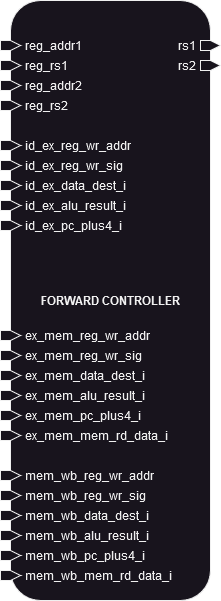
\includegraphics[width=0.35\textwidth]{design/pipelined/decode/images/forward_controller.png}
    \caption{Diagram of the Forward Controller}
    \label{fig:forward_controller}
\end{figure}

The forward controller is a module that is used to control what are the values used as rs1 and rs2 in the ALU. 
For example, if you have a data dependency between two instructions, the first one is a load and the second one is an add,
you need to forward the result of the load to the ALU. This module is responsible for that and instead of using the value of the register file,
it will use the value that is being forwarded. \\

Signals:
\begin{enumerate}[label={\textbullet}]
    \item Input: $reg_addr1$, This signal is representing the first register address that is being used by the current instruction.
    \item Input: $reg_rs1$, This signal is representing the value of the first register that is being used by the current instruction.
    \item Input: $reg_addr2$, This signal is representing the second register address that is being used by the current instruction.
    \item Input: $reg_rs2$, This signal is representing the value of the second register that is being used by the current instruction.
    \item Input: $id\_ex\_reg\_wr\_addr$, This signal is representing the register address that is being written by the previous instruction.
    \item Input: $id\_ex\_reg\_wr\_sig$, This signal is representing if the previous instruction is written to the register file or not.
    \item Input: $id\_ex\_data\_dest$, This signal is representing the origin of the data that is being used by the ALU in the previous instruction.
    \item Input: $id\_ex\_alu\_result$, This signal is representing the result of the ALU in the previous instruction.
    \item Input: $id\_ex\_pc\_plus4$, This signal is representing the pc plus 4 of the previous instruction.
    \item Input: $ex\_mem\_reg\_wr\_addr$, This signal is representing the register address that is being written by the previous instruction.
    \item Input: $ex\_mem\_reg\_wr\_sig$, This signal is representing if the previous instruction is written to the register file or not.
    \item Input: $ex\_mem\_data\_dest$, This signal is representing the origin of the data that is being used by the ALU in the previous instruction.
    \item Input: $ex\_mem\_alu\_result$, This signal is representing the result of the ALU in the previous instruction.
    \item Input: $ex\_mem\_pc\_plus4$, This signal is representing the pc plus 4 of the previous instruction.
    \item Input: $ex\_mem\_mem\_rd\_data$, This signal is representing the data that is being read from the memory in the previous instruction.
    \item Input: $mem\_wb\_reg\_wr\_addr$, This signal is representing the register address that is being written by the previous instruction.
    \item Input: $mem\_wb\_reg\_wr\_sig$, This signal is representing if the previous instruction is written to the register file or not.
    \item Input: $mem\_wb\_data\_dest$, This signal is representing the origin of the data that is being used by the ALU in the previous instruction.
    \item Input: $mem\_wb\_alu\_result$, This signal is representing the result of the ALU in the previous instruction.
    \item Input: $mem\_wb\_pc\_plus4$, This signal is representing the pc plus 4 of the previous instruction.
    \item Input: $mem\_wb\_mem\_rd\_data$, This signal is representing the data that is being read from the memory in the previous instruction.
    \item Output: $rs1$, This signal is representing the value that should be used as rs1 in the ALU.
    \item Output: $rs2$, This signal is representing the value that should be used as rs2 in the ALU.
\end{enumerate}